%%==================================================
%% chapter03.tex for SJTU Master Thesis
%% Encoding: UTF-8
%%==================================================

\chapter{FlexCore:采用VCPU-Ballooning的虚拟机动态调度系统}
\label{chap:flexcore}



\section{引言}

近年来,云计算平台由于其稳定、灵活、高效的特点, 逐渐受到了企业界的青睐,其通过网络以服务的方式提供可伸缩的虚拟计算资源,相比以往方式具备明显优势。而虚拟化技术作为云计算中最重要的核心技术之一,为其提供了基础架构层面的支持,成为了学术界研究的焦点。

而随着硬件技术的发展,处理器单个核心的性能提升逐渐遇到了瓶颈,处理器开始朝着多核化的方向演进,具备多个核心的处理器在云计算平台服务器上得到普及。为了充分利用多核处理器的并行性,与此同时满足用户对于处理能力的更高要求,具备多个虚拟处理器(Virtual CPU,vCPU)的虚拟机在实际生产环境中被广泛采用。而通过将多台虚拟机整合到一台物理机上运行,云服务提供商可以进一步提高硬件资源利用率并降低能源消耗成本。因此,如何提高整合后多台虚拟机的总体运行效率,成为了一个颇有实际价值的研究问题。

在虚拟化环境下,存在着双重调度现象[3],底下虚拟机监控器(Virtual Machine Monitor,VMM)将vCPU调度到物理处理器上,上层虚拟机中的操作系统再将里面运行的进程调度到vCPU上。然而,上层虚拟机中的绝大部分操作对于底下VMM而言是透明的,VMM中的调度器难以获知上层虚拟机中的真实运行情况。这层语义隔阂的存在,带来了一些在非虚拟化环境中不存在的问题,造成虚拟机中程序运行效率的低下。例如,虚拟机中一个持有内核自旋锁的vCPU在关闭内核抢占进入临界区的情况下,仍有可能因为处理器时间片耗尽或者物理机外部中断到来等原因被抢占。此现象将严重增加同步操作的延迟,因为另一个vCPU有可能在等待进入同一临界区。此问题在运行并行应用程序的多核虚拟机上将得到放大,严重阻碍了系统整体性能的提升。

但是,现有虚拟化平台采用的调度器并没有考虑到上述双重调度引发的性能问题。为此,以往研究者提出了若干种类似协同调度的策略[4][10],让相互构成协作关系的vCPU同时运行。然而,这些调度策略可能引入处理器时间碎片化和优先级反转等新问题,并没有将双重调度问题完全解决,给系统带来的整体性能改善也较为有限。

针对双重调度带来的性能下降,在前期的工作中[9]我们提出了vCPU-Ballooning方法(以下简称vCPU-Bal)。vCPU-Bal作为一种新的虚拟机调度方法,通过在运行时动态调整系统每个虚拟机中vCPU的数目,让每个vCPU在物理处理器上独占运行,降低多个vCPU因为争抢物理处理器而造成的性能损耗,提高系统的整体运行效率。其在本质上是弱化了VMM调度器的职责,将双重调度转化为一层,交予上层虚拟机。另由于现代云计算服务器往往具备几十甚至上百个物理处理器,vCPU-Bal这种调度方法在众核平台上是完全可行的。但是,[9]中仅仅说明了vCPU-Bal方法的初步构想,而本文阐述的FlexCore则给出了vCPU-Bal在KVM平台上的完整实现。经实验测试,在一台12核的服务器上,FlexCore在运行PARSEC测试套件时取得了约50\%的平均性能提升。

以下是本章的行文安排,第二节详述了虚拟化环境中的双重调度问题以及造成性能低下的两个原因,第三节介绍了FlexCore系统的设计与实现,第四节对FlexCore系统进行了性能测试,第五节是对相关研究工作的介绍,最后是对未来工作的展望和本章总结。



\section{背景介绍及问题分析}

\subsection{常见SMP虚拟机的调度方案}

每个SMP虚拟机均具备两个或多个vCPU,在确保隔离性的前提下允许用户同时使用多个CPU的计算资源,适合运行并行应用程序。在多个VM整合运行的场景中,一个物理CPU有可能被多个来自不同VM的vCPU共享,底下VMM中的调度器会根据每个vCPU的权重(share)来为其分配时间片。为了保证不同VM之间的公平性,VMM先将相同的share赋予系统中的每一个VM,再对每一个VM将share在其所有vCPU上平均分配。在每次发生上下文切换时,调度器会根据该vCPU在上个调度轮次内运行时间的长短来对其share进行更新。此外,在多核系统上,出于性能因素考虑,VMM为每个物理CPU维护了一个独立的调度器。为了维持物理CPU间负载的均衡,VMM会不定期地将vCPU从繁忙CPU迁往空闲CPU。

然而,由于虚拟化技术自身的原因,VMM中的调度器对上层VM中运行的实际情况知之甚少。这层语义隔阂的存在可能使得VMM中的调度器做出不友好的调度行为,例如让正在进行关键操作的vCPU被抢占或者得不到及时调度,造成VM中应用程序性能的严重下降。

\subsection{客户虚拟机CPU时间耗费情况分析}

为了验证以上结论,图\ref{fig:totaltime}比较了在一个VM单独运行(1VM)和两个VM同时运行(2VM)的配置下,VM中应用程序的运行时间。测试在一台具有12个物理CPU的服务器上进行,选取了PARSEC测试套件中的四个程序,每个VM均配备了12个vCPU和8GB内存。测试结果显示,尽管在两个VM同时运行的配置下,每个VM仅可以分到一半的计算资源,其总运行时间却分别达到了一个VM单独运行时的3.2倍、4.1倍、2.7倍和2.6倍(图\ref{fig:totaltime}每项左方实心柱体),另外其花在内核态的时间分别达到了后者的3.7倍、8.7倍、9.0倍和6.3倍(图\ref{fig:totaltime}每项右方空心柱体)。

\begin{figure}[!htp]
  \centering
  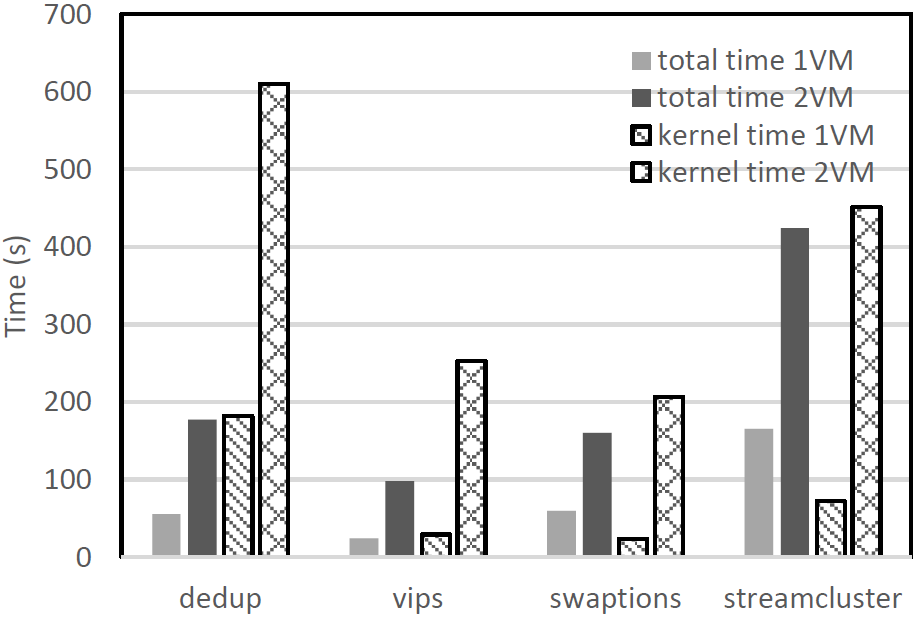
\includegraphics[width=0.7\textwidth]{chap4/total_time}
  \bicaption[fig:totaltime]{不同配置下总运行时间和内核态运行时间的比较}{不同配置下总运行时间和内核态运行时间的比较}{Fig}{Comparison on total execution time and kernel time between 1VM case and 2VM case}
\end{figure}

为了弄清VM中程序性能下降的原因,我们利用perf[6]工具对其进行了函数级别的采样分析(由于内核在编译时对spinlock进行了内联优化,此处借用了[5]中提及的lockstat方法测量其占用时间),结果如图\ref{fig:breakdown}所示。可以看到,大量的CPU时间消耗在函数调用IPI和spinlock自旋上,严重挤占了本应花费在有效工作上的时间,此为造成并行应用程序性能严重下降的主要原因。以下两节分别对函数调用IPI延迟和自旋锁持有者抢占进行详细分析。

\begin{figure}[!htp]
  \centering
  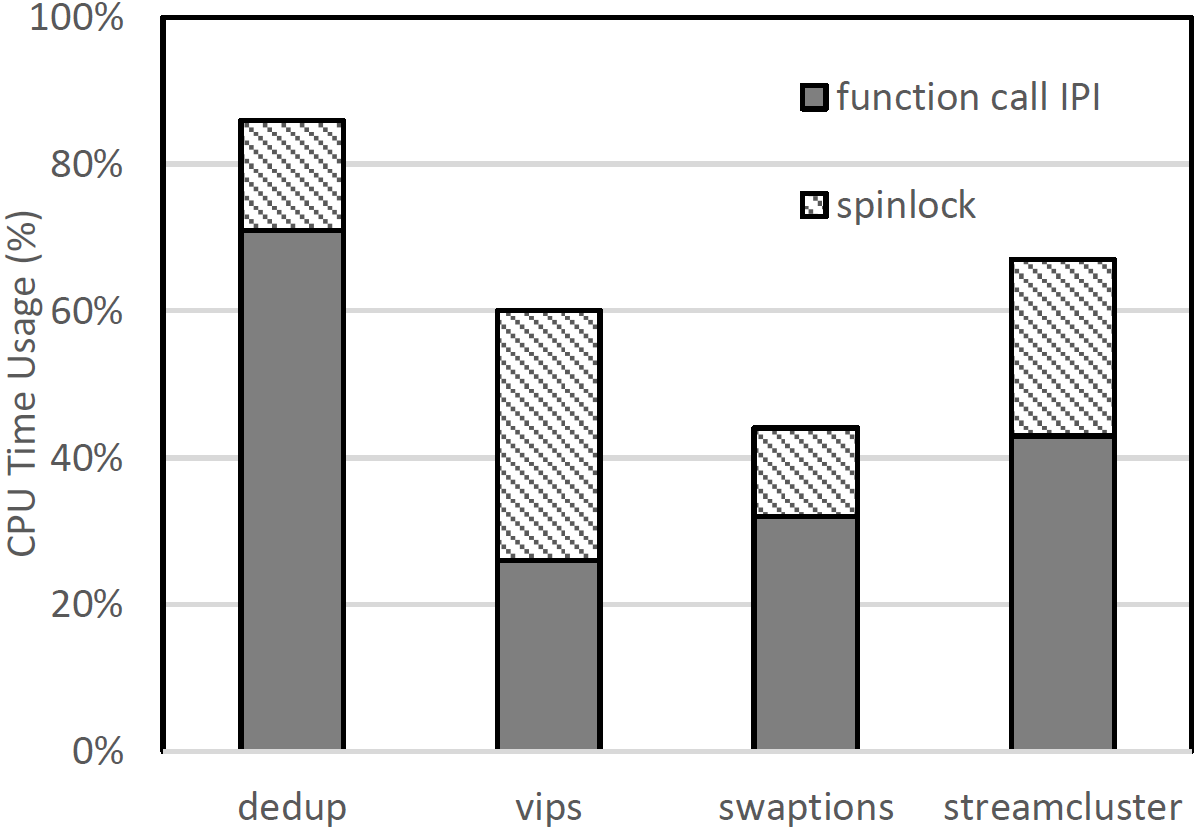
\includegraphics[width=0.7\textwidth]{chap4/breakdown}
  \bicaption[fig:breakdown]{2VM配置下应用程序总运行时间分解}{2VM配置下应用程序总运行时间分解}{Fig}{Breakdown on total execution time in 2VM case}
\end{figure}

\subsection{函数调用IPI延迟}

处理器间中断(Inter-Processor Interrupt, IPI)在SMP内核中被广泛使用,用于通知其他CPU某特定事件的发生,并要求后者执行相应操作,如TLB失效IPI和重新调度IPI。在Linux的实现中,函数调用IPI的发起者在中断发送后将一直处于忙等状态,直到所有的接收者对相应处理函数的调用完成。这种自旋忙等在真实物理硬件上是高效的,因为基于硬件的IPI具有低延迟和高优先级的特性,能保证处理函数在IPI接收者上迅速调用完成。

然而,在虚拟化环境中,IPI的实现需要通过VMM中的vAPIC来模拟。vCPU通过写vAPIC的MSR寄存器来告知VMM其发送行为,而IPI只有等到其接收者下一次获得调度前才能被注入。在多VM整合运行的情形下,每个CPU上的运行队列中可能有多个vCPU在等待运行,IPI的接收者往往不能被及时调度,这使得IPI的发送者必须进行相当长时间的自旋忙等。而函数调用IPI的接收者经常有多个,进一步加剧了这种忙等现象,大量浪费了CPU时间。如图\ref{fig:ipi_delay}所示,vCPU0在T1时刻向VM中其他vCPU广播了函数调用IPI,然后便开始自旋忙等。但由于此时其他CPU上已有vCPU在运行,vCPU1和vCPU2均未能被立即调度,vCPU0的忙等状态会一直持续到T2时刻,直到vCPU2经过$T_{schedule\_delay}$调度延迟接受IPI中断注入并完成处理函数。自此,在vCPU0上有$T_{busy\_waiting}$的时间耗费在了无用忙等上。

\begin{figure}[!htp]
  \centering
  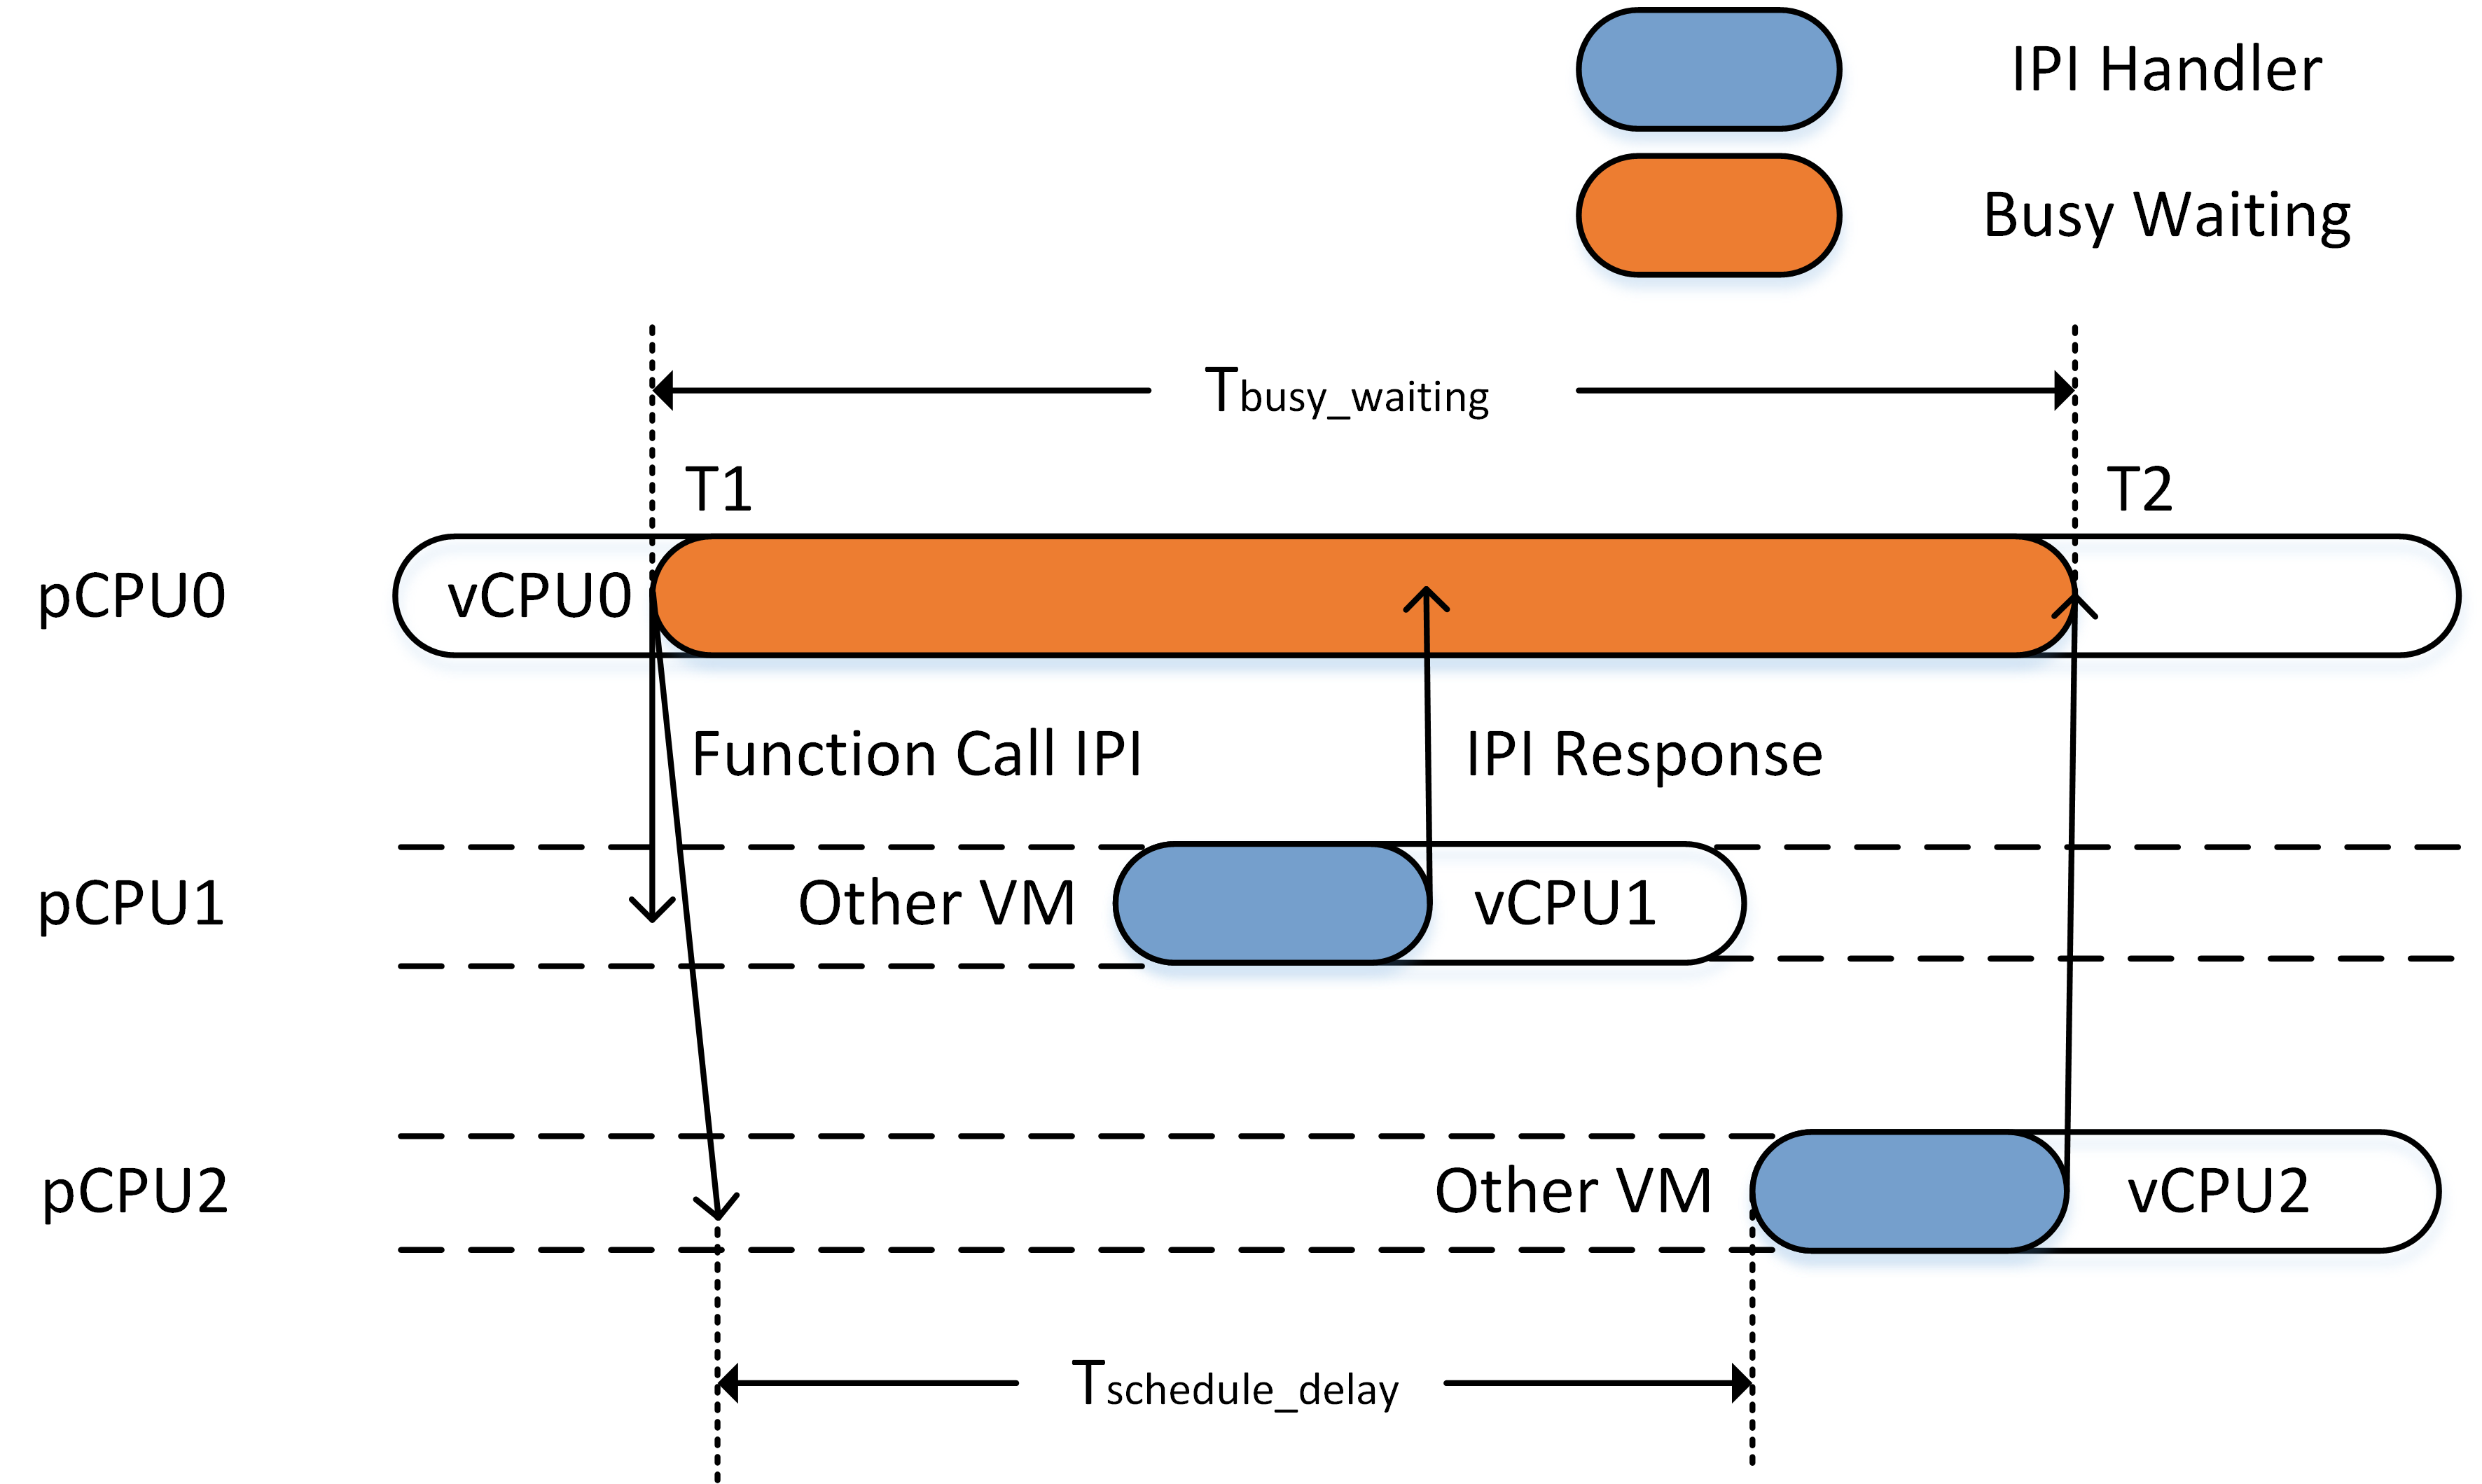
\includegraphics[width=0.7\textwidth]{chap4/ipi_delay}
  \bicaption[fig:ipi_delay]{函数调用IPI延迟示意图}{函数调用IPI延迟示意图}{Fig}{Illustration on function call IPI delay}
\end{figure}

\subsection{自旋锁持有者抢占}

在内核中自旋锁被用于多CPU间的同步,防止出现竞态条件,CPU在拿锁之前自旋等待。自旋锁的临界区一般较短,只有几十个时钟周期,在真实硬件上,这是一种高效的同步原语。

但在虚拟化环境中,自旋锁的同步延迟有可能增大。尽管锁的持有者在进入临界区前关闭了内核抢占,其对应的vCPU仍有可能因为处理器时间片耗尽或物理机外部中断到来等原因被抢占。与此同时,该VM中其他vCPU可能因为在等待进入同一临界区,而不得不一直自旋,直到锁的持有者被重新调度退出临界区。如\ref{fig:spinlock}所示,持有自旋锁的vCPU0在进入临界区后于T1时刻被抢占,与此同时位于pCPU1上的vCPU1也在等待进入同一临界区。由于始终未能成功拿锁,vCPU1的自旋状态持续到T2时刻,直到vCPU0经过$T_{preempt}$的时间被重新调度并完成工作退出临界区。自此,vCPU1上该自旋锁的同步延迟被放大至$T_{lock\_wait}$,期间也有大量时间耗费在无用自旋上。

\begin{figure}[!htp]
  \centering
  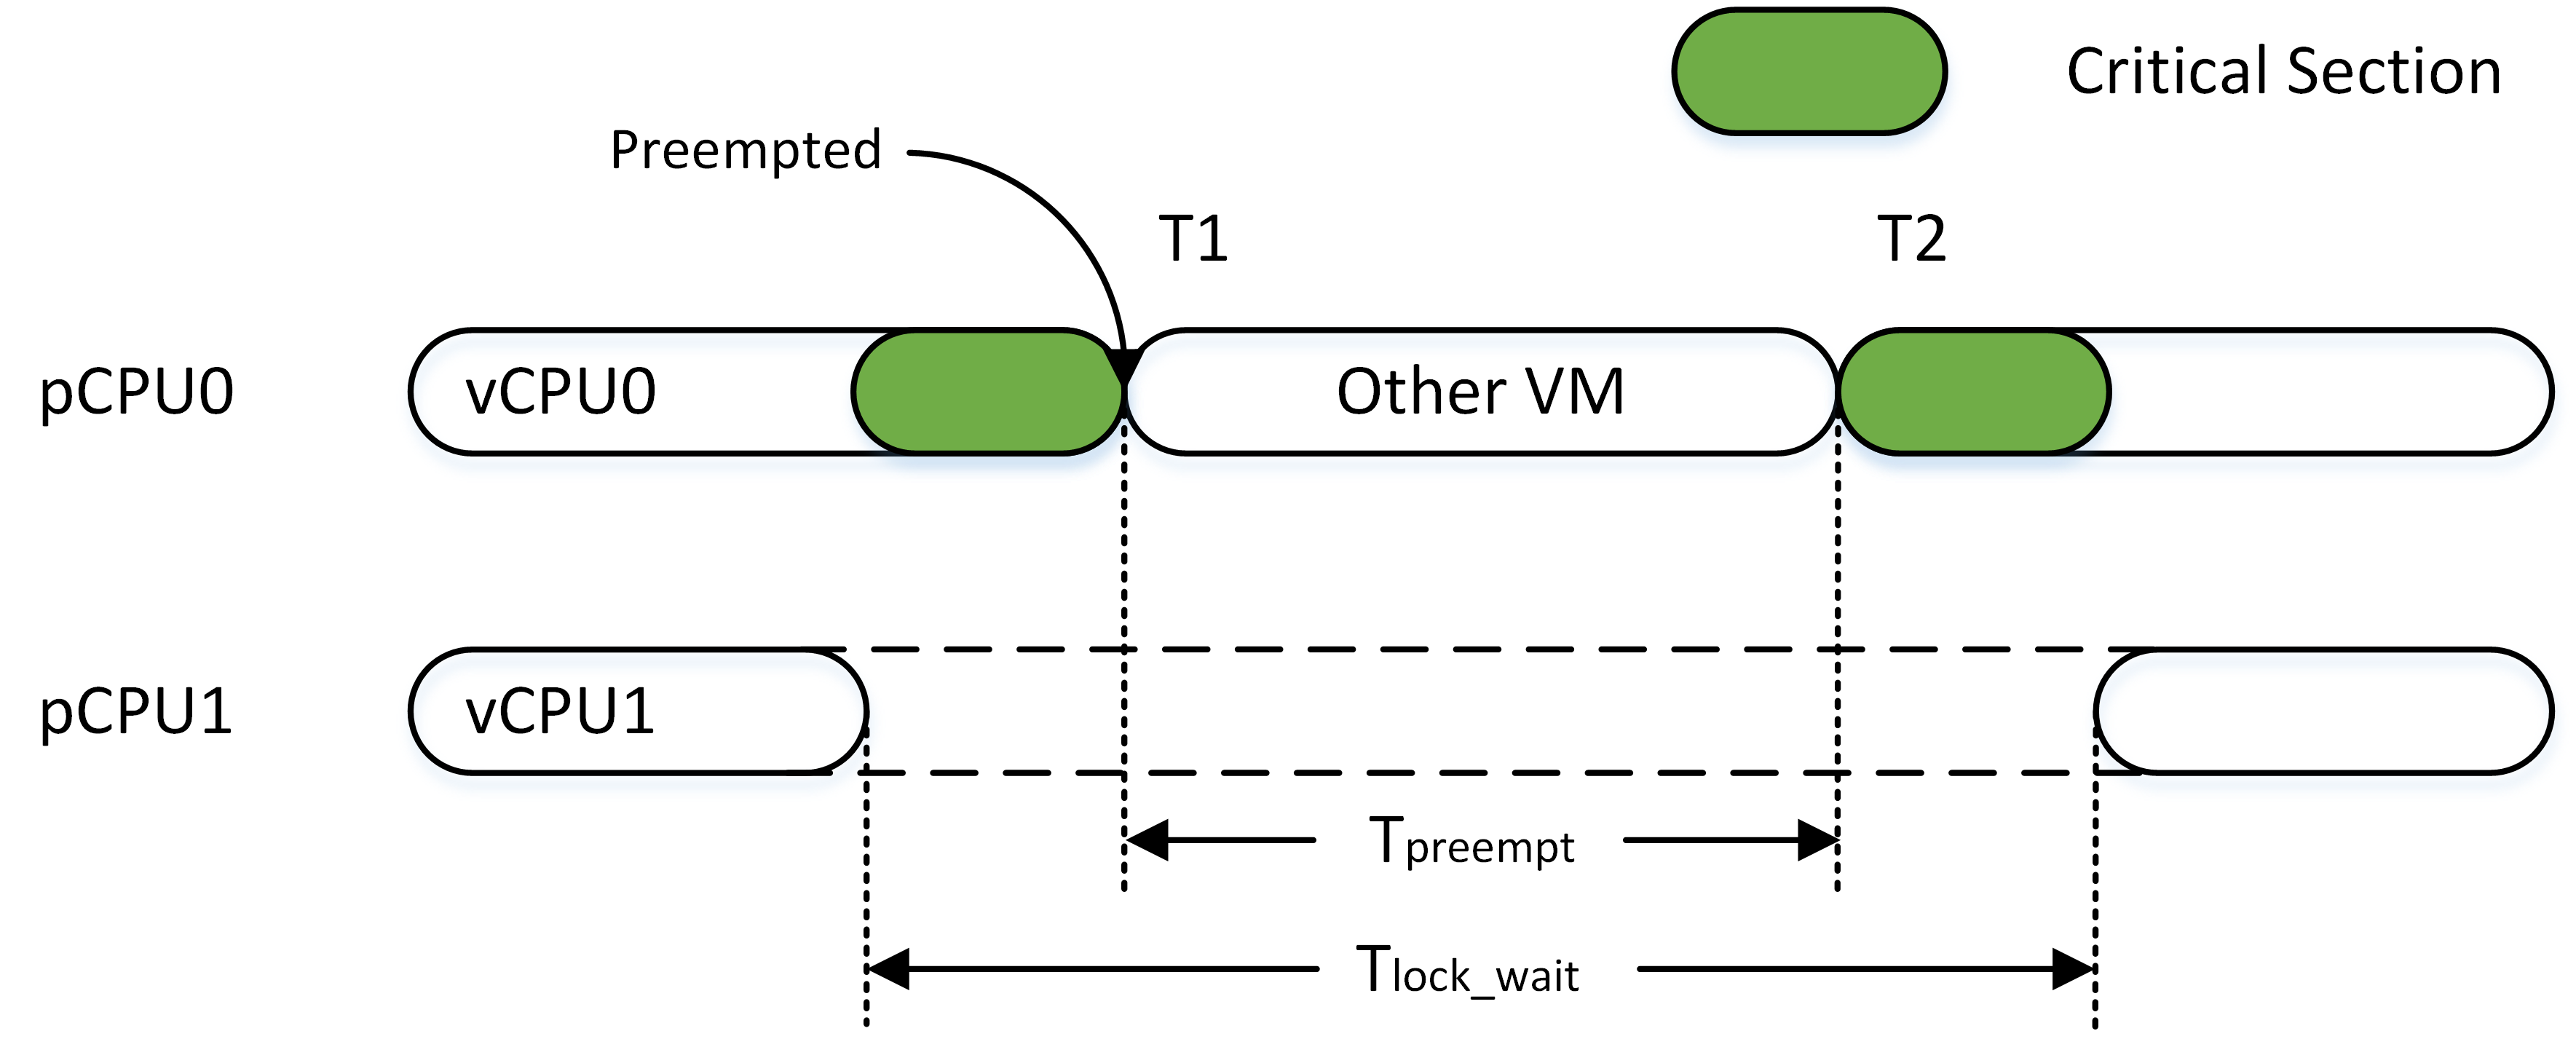
\includegraphics[width=0.7\textwidth]{chap4/spinlock}
  \bicaption[fig:spinlock]{自旋锁持有者抢占示意图}{自旋锁持有者抢占示意图}{Fig}{Illustration on spinlock holder preemption}
\end{figure}

\subsection{vCPU-Bal方法}

以上两种现象,均可视为由于语义隔阂的存在,VMM中的调度器不清楚VM的实际运行状况,而盲目做出的不友好调度行为所导致的。对于函数调用IPI延迟,VMM未能将IPI的接收者及时调度,造成发送者在等待结果上耗费了大量时间。对于自旋锁持有者抢占,VMM将仍处于临界区中的vCPU抢占,使得其他vCPU在等待拿锁时长时间自旋。双重调度的存在,让大量CPU时间花在了无用操作上,严重降低了VM中应用程序的性能。

由于虚拟化技术自身所限,VM中的大部分操作对VMM透明,VMM调度器难以获取足够的信息来做出恰当的调度行为。针对此双重调度的困境,vCPU-Bal从一个全新的角度来解决问题,通过弱化VMM的调度职责,将双重调度转化为一层调度。其能够在运行时动态调整VM中vCPU的数目,让系统中每个vCPU都能独占CPU运行。自此,由于每个CPU的运行队列中仅有一个vCPU,在任何时刻该vCPU均可获得运行机会,IPI接收者便能迅速完成对处理函数的调用从而保证发送者尽快退出忙等,同理自旋锁持有者也可以尽早完成临界区执行从而避免其他等待拿锁者长时间自旋。

vCPU-Bal方法具有以下优点:

\begin{itemize}
\item{通过vCPU的独占运行,减轻函数调用IPI延迟和自旋锁持有者抢占,大量减少做无用操作的时间。}
\item{降低在不同vCPU间做上下文切换的开销,让CPU上的缓存和TLB在更长时间内有效。}
\item{避免VM操作系统自身在核数众多时的可扩展性瓶颈。}
\end{itemize}



\section{FlexCore系统的设计与实现}

因KVM[2]作为Linux的内核模块发布,便于安装调试,且在学术和商业中都有广泛应用,本文所述的FlexCore系统在此平台上实现。但由于vCPU-Bal方法并非与虚拟化平台的具体实现耦合,故该方法可以被运用在其他虚拟化平台上,如Xen[1]等。此外,VM中的操作系统也采用了Linux。

并行应用程序在FlexCore系统之上的一个典型执行过程由以下三个阶段组成:

1)vCPU ballooning前:由于vCPU上的工作负荷不重,vCPU之间的交互(竞争自旋锁或互发中断)也不多,客户虚拟机按照起先默认分配的vCPU数目运行。

2)vCPU ballooning中:随着越来越多的vCPU转为可运行状态,vCPU开始在物理核上竞争运行机会,vCPU之间的交互也越来越频繁,

3)vCPU ballooning后:

\subsection{系统总体架构}

\begin{figure}[!htp]
  \centering
  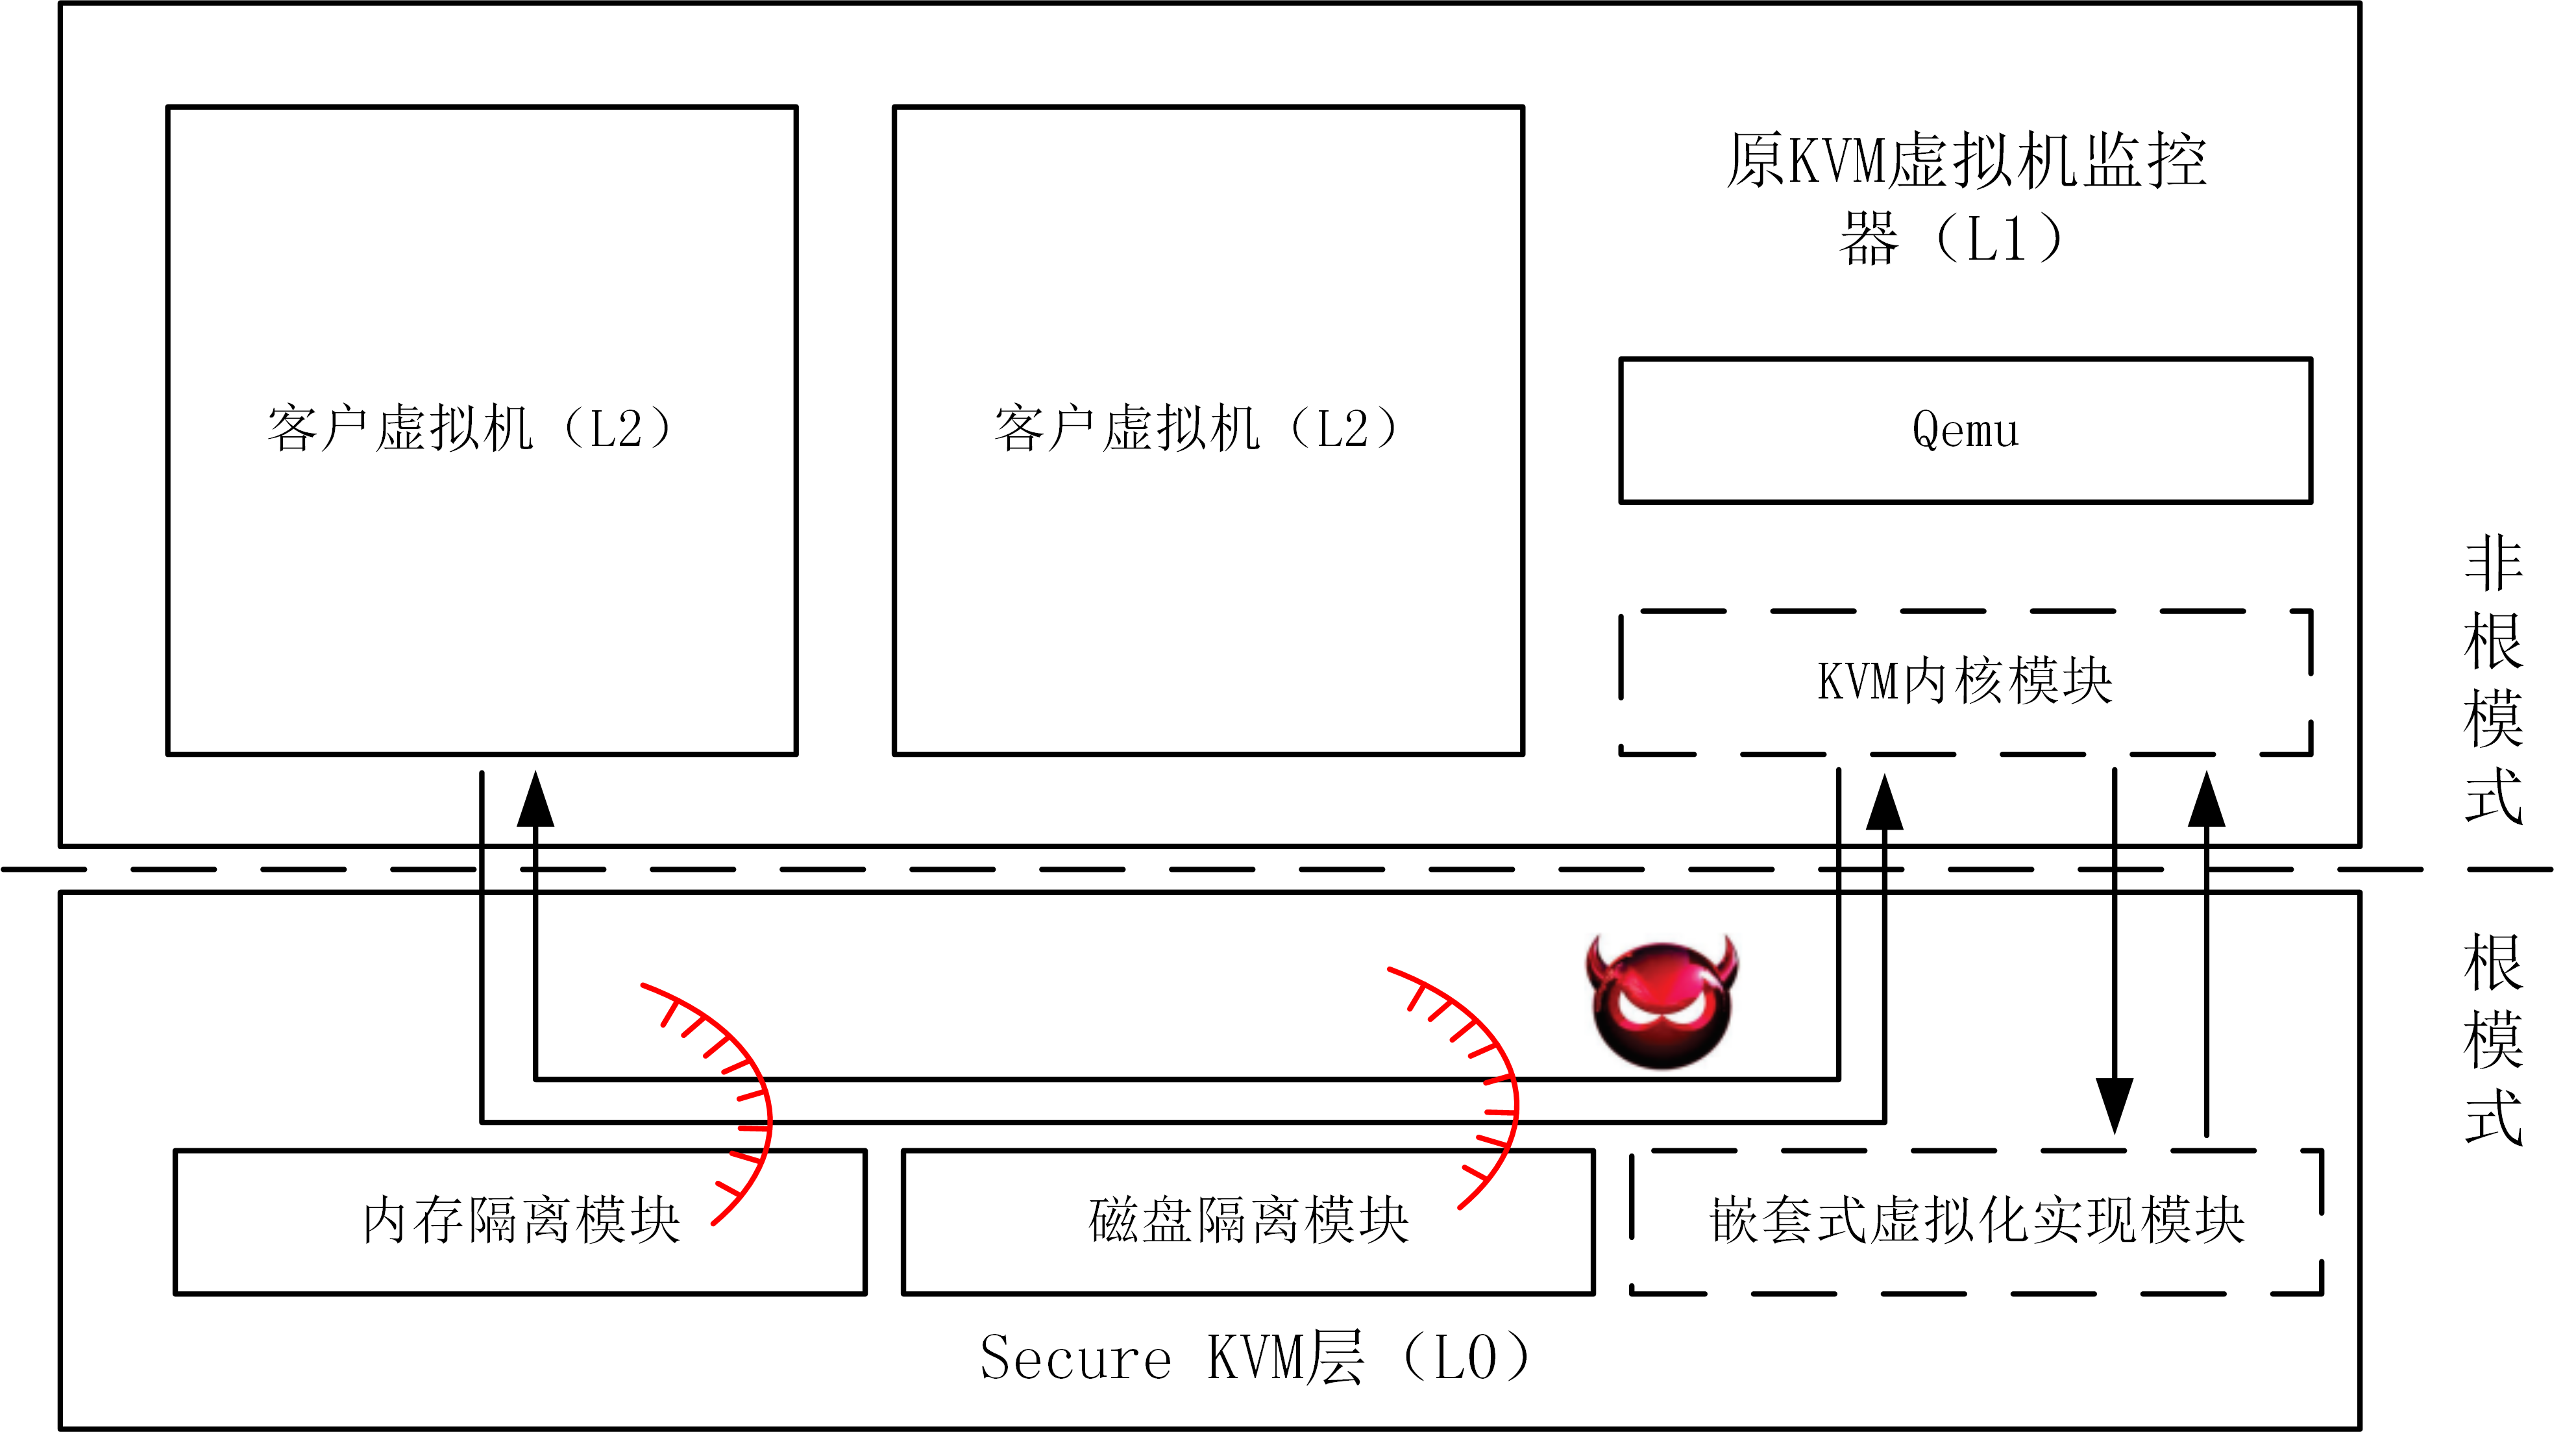
\includegraphics[width=0.7\textwidth]{chap4/architecture}
  \bicaption[fig:architecture]{KVM平台上FlexCore系统的总体架构}{KVM平台上FlexCore系统的总体架构}{Fig}{System architecture of FlexCore on KVM}
\end{figure}

图\ref{fig:architecture}展示了FlexCore系统在KVM平台上的总体架构,主要由VMM中的vCPU-Bal控制中心、VM中的vCPU-Bal内核代理以及两者之间通信模块三部分组成,以下三节分别对其做详细描述。

\subsection{vCPU-Bal控制中心}

vCPU-Bal控制中心位处VMM,它对系统中每个vCPU的实际运行情况进行统计,并据此发出vCPU-Bal和绑核指令。

Intel在其最新的支持硬件虚拟化的CPU中添加了暂停-循环退出(Pause-Loop Exiting,PLE)特性[12]。PLE定义了两个参数,一个是PLE\_Gap,指在一个自旋循环中两条pause指令相隔的CPU时钟周期数,另一个是PLE\_Window,指在发生虚拟机陷入(VMExit)前经过的自旋循环次数。在VM中一条pause指令发出时,如果相距上一条pause指令超过了PLE\_Gap,那么PLE就认为开始了一个新的循环,而如果没有超出,则进行次数累加,直到超过PLE\_Window即触发VMExit。

而无论是IPI发送者忙等接收者处理函数返回,还是vCPU在拿锁前自旋,其在实现中为了减少对CPU高速缓存行造成的竞争,在每次尝试失败后均会执行pause指令。如果其尝试失败次数超过PLE\_Window,在随后发生VMExit时便能被监测到。因此,一段时间内较高的PLE次数,可以说明系统有大量的CPU时间被耗费在双重调度导致的无用忙等上,此时应该用vCPU-Bal方法来缓解vCPU间的无谓竞争,提高系统的实际运行效率。

现阶段vCPU-Bal控制中心依据每个VM的权重来计算其应分配的vCPU个数。以下公式,具体说明了每个VM获分配vCPU数目$N_{vCPU}$的计算过程,其中$W_{VMi}$表示系统中第i个VM的权重,$T_{pCPU}$表示系统中所有物理CPU的个数。

\begin{equation*}
N_{vCPU} = \frac{W_{VMi} * T_{pCPU}}{\sum_{i=1}^n W_{VMi}}
\end{equation*}

假设某个12核系统中运行有两个VM,VM1和VM2均有12个vCPU,权重分别为512和256,那么vCPU-Bal控制中心将把VM1的vCPU数减少为8,把VM2的vCPU数减少为4。

\begin{figure}[!htp]
  \centering
  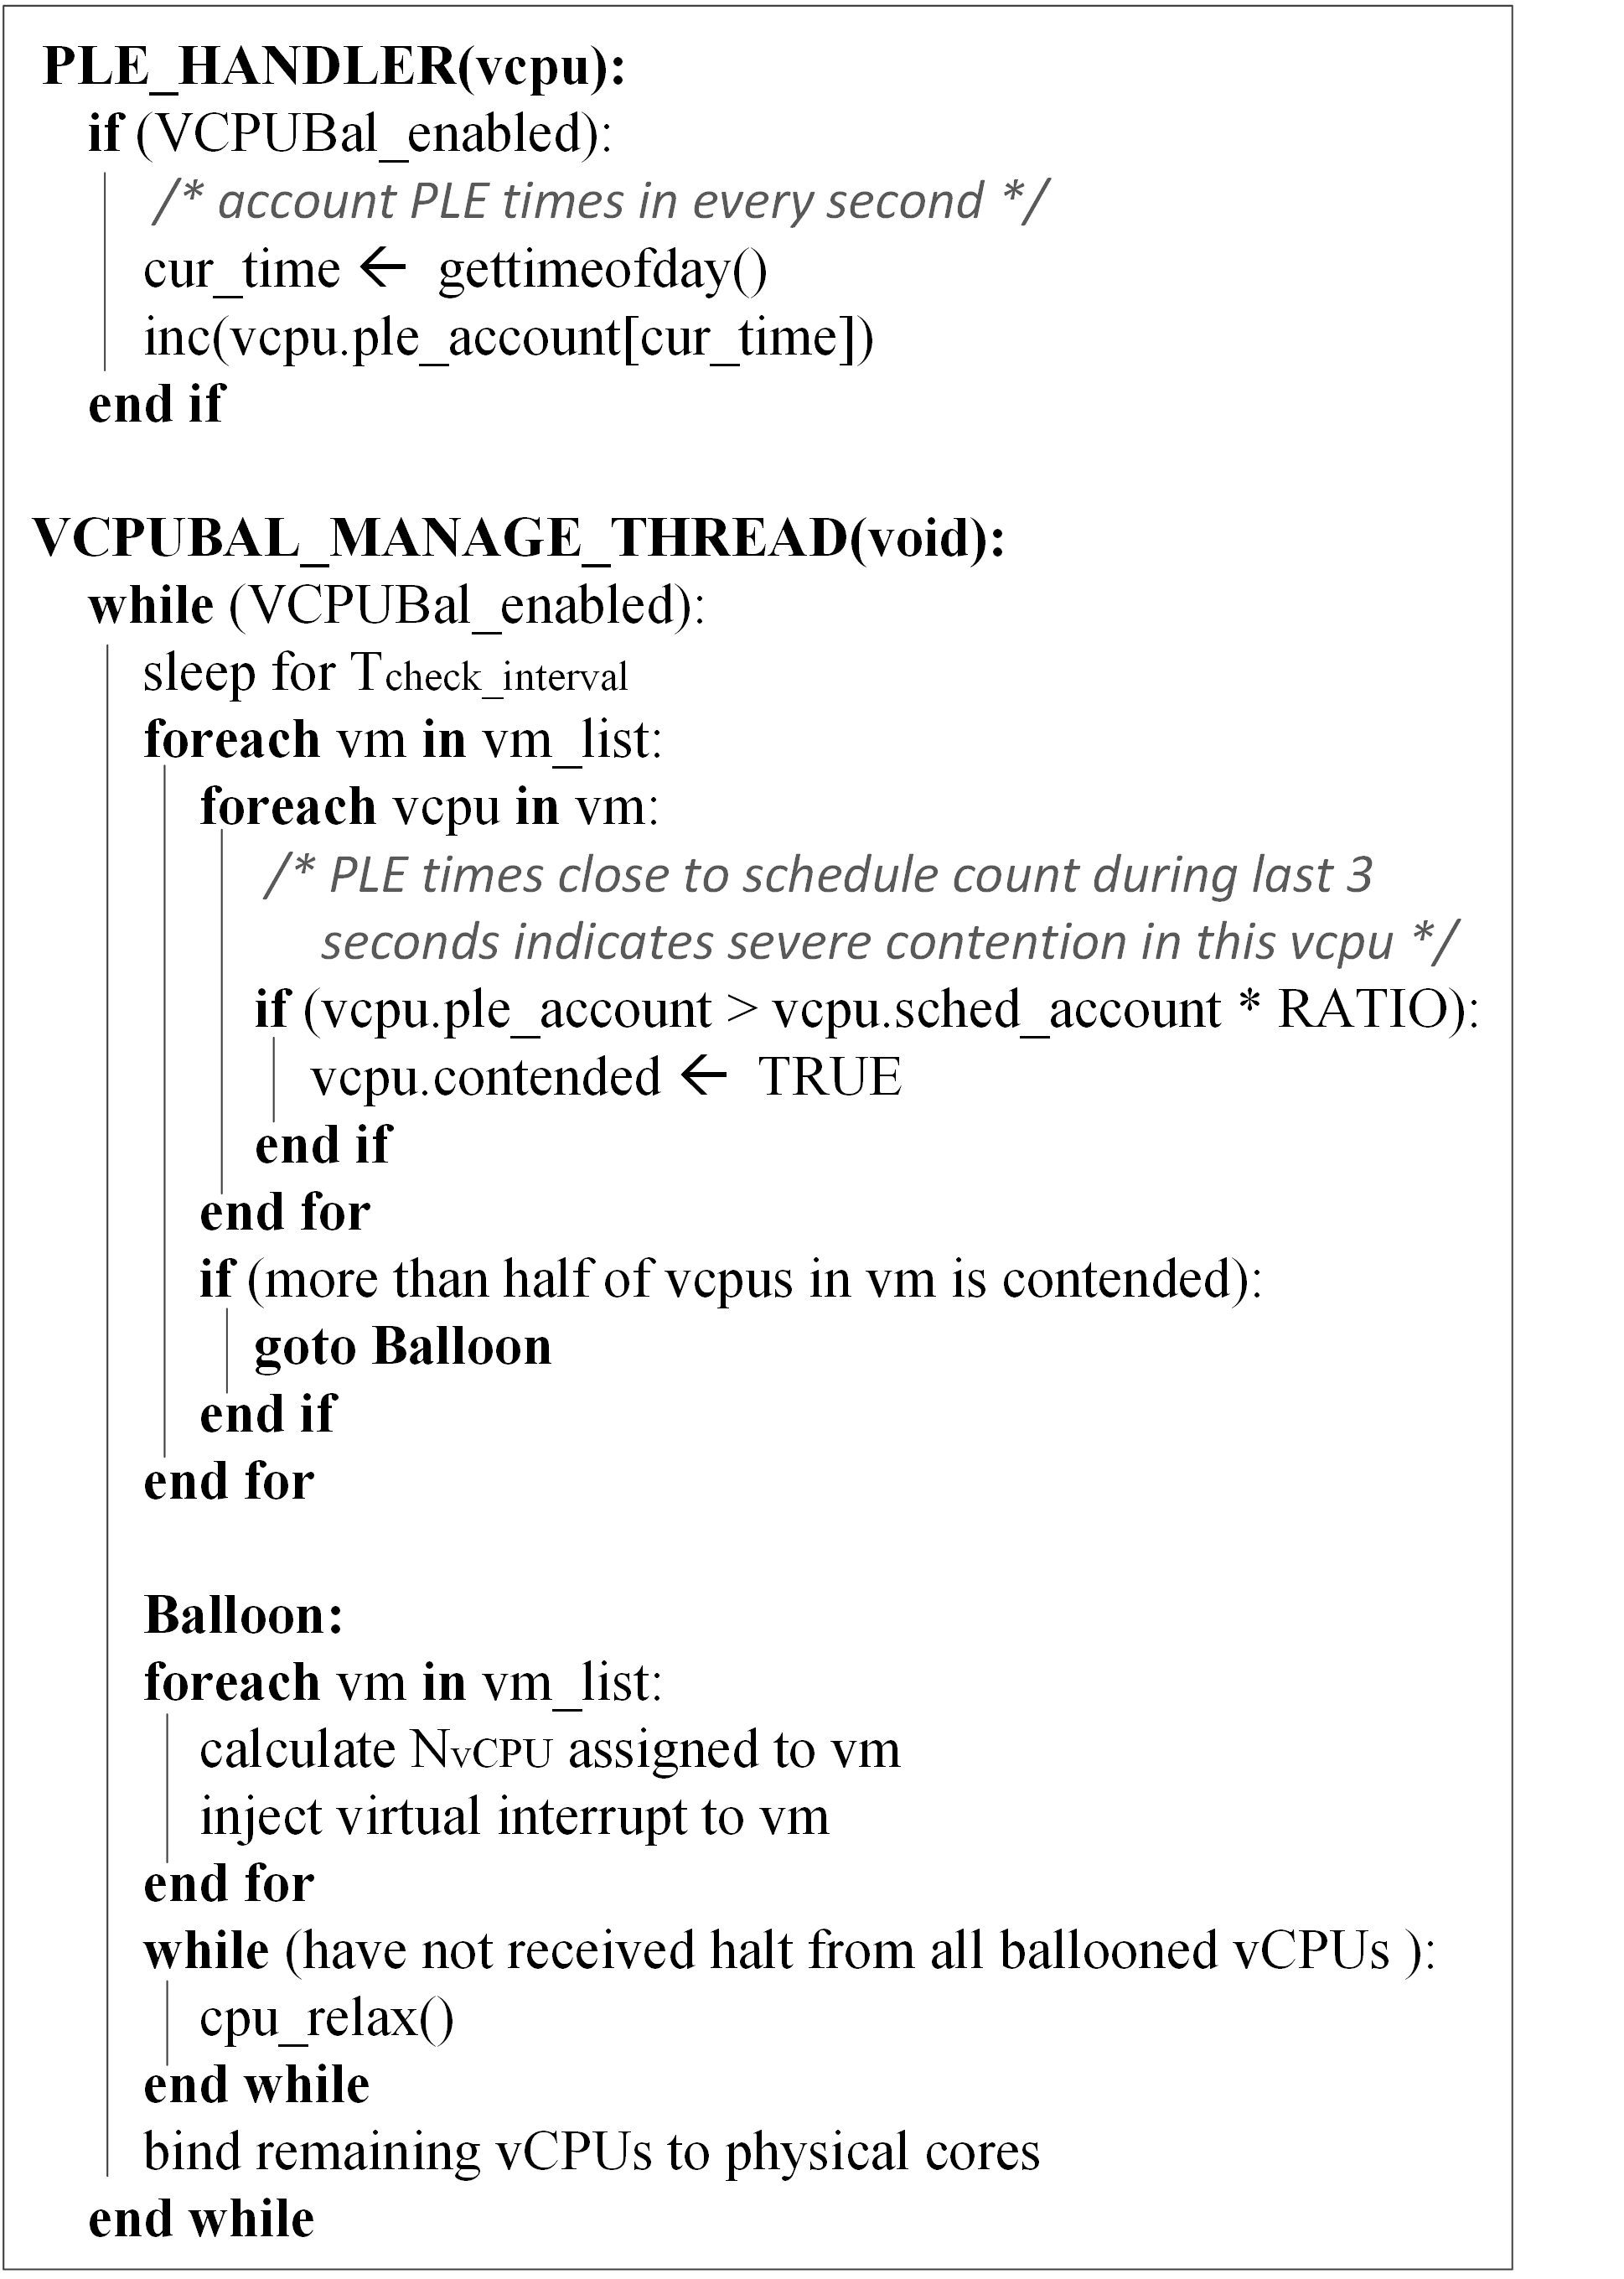
\includegraphics[width=0.8\textwidth]{chap4/algorithm}
  \bicaption[fig:algorithm]{vCPU-Bal基本流程伪代码}{vCPU-Bal基本流程伪代码}{Fig}{Algorithm in vCPU-Bal control center}
\end{figure}

\subsection{vCPU-Bal内核代理}

系统中每个VM均包含有vCPU-Bal内核代理。该代理会在VM启动后自行加载并与vCPU-Bal控制中心建立通信通道,等待后者发出的vCPU-Bal指令并执行,在运行时动态调整vCPU数目。

该内核代理在实现中有若干难点。首先,Linux中有众多的Per-CPU状态信息,如每个CPU独立访问的Per-CPU变量和绑核运行的Per-CPU内核线程。然后,Linux中一些子系统与当前在线CPU数目紧密关联,如IPI广播需要全局CPU的参与,又如RCU[14]在回收资源前经历的宽限期需要在所有CPU上发生一个上下文切换。

现阶段该内核代理利用Linux自带的CPU热插拔(CPU Hotplug)特性[13]来实现。在动态减少vCPU时,其首先将该vCPU在全局位图中标记为离线,这样IPI广播等需要全局vCPU参与的操作将会把该vCPU排除在外。然后,内核代理会等待一个宽限期以回收RCU释放的资源,因为此刻其他vCPU上可能的对这些资源的引用均已结束。随即内核代理暂停先前在该vCPU上运行的Per-CPU内核线程并将该vCPU运行队列中的其他普通线程迁移到其他vCPU,最后其调用各Linux子系统注册的回调函数并执行halt指令将该vCPU置于停机状态。而这条halt指令能触发VMExit,会被VMM监测到,vCPU-Bal控制中心据此判定该vCPU已被成功离线。

vCPU-Bal内核代理会优先离线编号较大的vCPU,如某VM中有0-11共计12个vCPU,而控制中心需要将其vCPU数减为6,内核代理会将以上流程在6-11vCPU上逐一运行。

\subsection{介于控制中心和内核代理间的通信模块}

VMM中的vCPU-Bal控制中心与VM中的vCPU-Bal内核代理需要进行双向通信,此功能由构建在他们中间的通信模块来完成。

为了达到目的,我们采用了类似XenStore[1]机制的方法,在KVM用作设备模拟的Qemu中添加了一个虚拟PCI设备,并在VM中为其编写了驱动。驱动初始化过程中会为该设备分配中断号,并预留两个内存页作为和vCPU-Bal控制中心之间的共享内存。驱动初始化完成后,该中断号和内存页物理地址将通过带特殊参数的vmcall[12]指令告知VMM,VMM随即将内存页映射至其地址空间,通信通道自此建立完成。

若vCPU-Bal控制中心欲发送消息给vCPU-Bal内核代理,其可以将消息内容写入第一个内存页,并以注入虚拟中断的方式来通知VM。反之,vCPU-Bal内核代理可以将消息内容写入第二个内存页,并执行带特殊参数的vmcall指令来通知VMM。



\section{实验与性能测试}

\subsection{实验环境}

\subsection{总运行时间比较}

\subsection{运行时间占比比较}

\subsection{PLE次数比较}

\subsection{实验总结}



\section{相关研究工作分析}



\section{总结与展望}